\section{Introduction}
\label{sec:intro}
%Deep neural models have shown to be effective in 
%a large variety of natural language inference~(NLI)
%tasks~\cite{bowman2015large,wang2018glue,mostafazadeh2016corpus,roemmele2011choice,zellers2018swag}. Many of these tasks
%are discriminative by nature, such as choosing a class 
%or an outcome from multiple choices, as shown in the following example:

Deep neural models have shown to be effective in a large variety of natural language
understanding (NLU) tasks~\cite{bowman2015large,wang2018glue,mostafazadeh2016corpus,roemmele2011choice,zellers2018swag} that often involve discriminating between 
%Large language models (LLMs) like ChatGPT~\footnote{\url{https://chat.openai.com/}}, 
%released by OpenAI, can solve various natural language processing (NLP) 
%tasks zero-shot, without task-specific training data, by using suitable prompts. 
%Before LLMs, deep neural models excelled in natural language 
%inference (NLI) tasks
categories or outcomes in multiple-choice settings, as demonstrated in~\exref{exp:snli}. 
However, accurately evaluating these models is crucial, 
as many exhibit fragility when faced with minor perturbations~\cite{checklist2020acl}.
\begin{center}
\fbox{
    \begin{minipage}{\textwidth}
\begin{example}\label{exp:snli}
Natural language inference in SNLI dataset, with ground truth bolded.
\begin{description}
\item{Premise:} A swimmer playing in the surf watches a low flying airplane headed inland. 
\item{Hypothesis:} Someone is swimming in the sea.
\item{Label:} \textbf{a) Entailment.} b) Contradiction.  c) Neutral.
\end{description}
\end{example}
    \end{minipage}
}
\end{center}

Humans solve problems by reasoning about logical connections 
between premises and hypotheses. 
Some NLP models~\cite{naik2018stress,schuster2019towards}, 
however, can solve problems by merely observing dataset hypotheses. 
This may occur because hypotheses are often artificially 
written and contain human biases predictive of correct answers. 
We call such biases artificial spurious \textit{cues} when
they appear both in the training and test datasets with a similar distribution
over the prediction values, which is illustrated in~\figref{fig:cue_def}.
These biases can manifest as statistical correlations, 
such as sentiment, repeated words, or shallow n-grams. 
When models rely on these biases, or cues, 
their performance may be negatively affected 
when these cues are removed, indicating a lack of robustness.

%The number of candidate labels may vary. Humans solve such questions by
%reasoning the logical connections between the premise and the hypothesis,
%but previous work~\cite{naik2018stress,schuster2019towards} 
%has found that some NLP models can solve the questions
%fairly well by looking only at the hypothesis (or ``conclusion'' in some work)
%in the datasets.
%It is widely speculated that this is because, in many datasets, 
%the hypotheses are manually crafted and may contain artifacts that
%would be predictive of the correct answer. 
%Such ``hypothesis-only'' tests can identify problematic questions
%in the dataset if the question can be answered correctly without 
%the premise. While such a method to evaluate the quality of
%a dataset is theoretically sound, 
%it i) usually relies on training a heavy-weight model such as Bert, which
%is costly to evaluate, ii) does not provide an explanation of why the question is 
%a culprit, and iii) cannot be used to evaluate a model since a model that
%can make a correct prediction using only the hypothesis is not necessarily a
%bad model: it is just not given the complete data.  

\begin{figure}[th]
\centering
\includegraphics[width=0.45\columnwidth]{picture/cue_def.eps}
\caption{Example of a {\em cue}. }
%\KZ{``Possible distributions of the same feature''}}
\label{fig:cue_def}
\end{figure}

As we mentioned above, ``hypothesis-only'' tests can identify dataset issues 
when questions can be answered correctly without the premise.
However, they cannot validate the model's ability to answer questions without a 
premise due to 
%a) it relies on training heavyweight models (like BERT) and is costly, 
a) it doesn't explain the cause of the model's problems, 
and b) it doesn't directly evaluate the model, 
as models use complete data during training and prediction, 
making ``hypothesis-only'' tests unrealistic.

Inspired by black-box testing in software engineering, 
CheckList~\cite{checklist2020acl} 
assesses model weaknesses without requiring detailed knowledge 
of the model by providing additional stress test cases based 
on predefined linguistic features. 
However, CheckList has limitations due to 
the need for carefully crafted templates with 
substantial restrictions, which limits the 
testing space and complicates implementation. 
Moreover, while CheckList identifies what the model cannot do, 
it fails to shed light on what the model has actually learned from the data.

%Inspired by black-box testings in software engineering, 
%CheckList~\cite{checklist2020acl} assesses the weakness of 
%models without the need to know the details of the model. It does so by
%providing additional stress test cases according to predefined 
%linguistic features. Unfortunately, to ensure the correctness of
%these additional cases, the templates must be carefully crafted
%with substantial restrictions, thus limiting the testing space and
%complicating the implementation. 
%Furthermore, with CheckList, you only get to know what the model 
%is incapable of doing but won't know what the model has 
%learned from the data.
%
%While ChatGPT has surpassed many previous deep neural models in various tasks and has some self-explanatory abilities, we find that ChatGPT's self-explanation in commonsense reasoning tasks is not clear enough. It cannot reveal the reasons for making choices or judgments in commonsense reasoning tasks, nor can it self-verify whether it is biased by data distribution, as with other natural language understanding (NLU) models.

%Inspired by black-box testing in software engineering, CheckList~\cite{checklist2020acl} assesses model weaknesses without needing detailed knowledge of the model. It provides additional stress test cases based on predefined linguistic features. However, ensuring the correctness of these cases requires carefully crafted templates with substantial restrictions, limiting the testing space and complicating implementation. Moreover, CheckList only reveals what the model cannot do without shedding light on what the model has learned from the data.

To address the above limitations of existing approaches and 
fully utilize existing test sets, we propose ICQ (``I-see-cue''), 
a lightweight, general statistical analysis framework. 
ICQ identifies biases in multiple-choice NLU datasets 
without the need for additional test cases and evaluates 
how models exploit these biases through black-box testing. 
As an open-source evaluation framework~\footnote{\url{http://anonymized.for.blind.review}}, 
ICQ allows for the assessment of both datasets and their 
corresponding models by extracting multiple test sets 
from different perspectives within a single dataset.

We validate ICQ's effectiveness on various NLU datasets 
to investigate whether models have learned potential bias 
information during training. 
By employing the ICQ framework, 
we gain a better understanding of ChatGPT~\footnote{\url{https://chat.openai.com/}}'s 
learning of potential biases and discuss, 
through examples, how to select appropriate prompts, 
ultimately providing 
valuable guidance for model optimization.


%In this paper, our view is that the existing test sets for these
%tasks are not sufficiently exploited. Why do we go the extra mile to
%generate new test cases which are potentially incorrect, when we can
%test the models using existing test sets but from different perspectives?
%With this objective in mind, we propose ICQ 
%(``I-see-cue''), an open-source evaluation 
%framework~\footnote{\url{http://anonymized.for.blind.review}} for 
%evaluating both the dataset and the corresponding models. In this framework, 
%one test dataset can be extracted into multiple test sets from different perspectives. 
%
%Previous studies~\cite{gururangan2018annotation,sanchez2018behavior,poliak2018hypothesis} 
%showed that statistical bias on linguistic features 
%(e.g., sentiment, repetitive words, and even shallow n-grams)
%which have a statistical correlation with specific labels 
%in benchmark datasets can be predictive of the correct 
%answer. We call such biases artificial spurious \textit{cues} when
%they appear both in the training and test datasets with a similar distribution
%over the prediction values.
%We illustrate this in~\figref{fig:cue_def}. 
%Once these cues are neutralized from the test data, 
%previously successful models may degrade substantially
%on it, suggesting that the model has taken advantage of 
%the biased feature and is hence not as robust as assumed 
%against such cues.
%

In summary, this paper makes the following contributions:
%\KZ{These contribs need to be revised right?}
\begin{itemize}
%\item we provide a lightweight but effective method to reveal statistical biases and cues in NLU datasets;
%(\secref{sec:result}).
%\item we propose two simple tests to quantitatively and visually
%assess whether a given model has taken advantage of a
%spurious cue when making predictions;

\item we present a lightweight yet effective method to uncover statistical biases and cues in NLU datasets, and propose two simple tests for quantitatively and visually evaluating whether a given model exploits spurious cues in its predictions.

\item we conduct a comprehensive evaluation of statistical bias issues on 10 popular NLU datasets and 4 models, confirming previous findings and uncovering new insights, while also providing an online demonstration system to showcase the results and encourage users to assess their own datasets and models.
%\item we make comprehensive evaluation of statistical bias issues on 10 popular NLU datasets and 4 models, confirming previous findings and discovering new insights;
%\item we created an online demonstration system to showcase
%the results and invite users to evaluate their own datasets and models.
%\item we showcase a case study on selecting prompts that can investigate ChatGPT's bias, 
%providing useful recommendations for practical applications.
%\item we make a case study of how to select prompts that can reduce ChatGPT's bias, 
\item we investigate ChatGPT's bias through a case 
study and offer valuable recommendations for practical applications.

\end{itemize}
% (\secref{sec:result}).

%\item We filter the training data and get a better performance on the \textbf{hard} dataset.
%to get a high quality training dataset which
 %is possibly closer to the intended task. 







